\subsection{Interesting observation}

According to Figure \ref{figure:experiments:classification:accuracy-per-class-best}, two  models achieving the best validation accuracy, \textit{nn-2x-512-tanh-softmax} and \textit{nn-512-sigmoid-softmax}, demonstrate similar performance on every label.
However, it is interesting to observe that both models struggle with \textit{shirt}s. Although both models perform decently on \textit{pullover} and \textit{T-shirt}, they both perform significantly worse on \textit{shirt}. 

Figure \ref{fig:experiments:classification:best-tanh} demonstrates that the training and accuracy gap of \textit{nn-2x-512-tanh-softmax} remains quite small. However, in Figure \ref{fig:experiments:classification:best-sigmoid}, we can observe slightly larger gap between training and validation accuracy of \textit{nn-512-sigmoid-softmax}. Since the training accuracy of both models peaks at about $82 \%$, there is evidence to suggest both models struggle to fit the training set. Hence, there is no evidence that those networks overfit. In the previous section, we observed that the addition of more fully-connected layers does not significantly affect the generalization. This may indicate that fully-connected architecture is generally too simple for this dataset.


\begin{figure}[H]
    \centering
    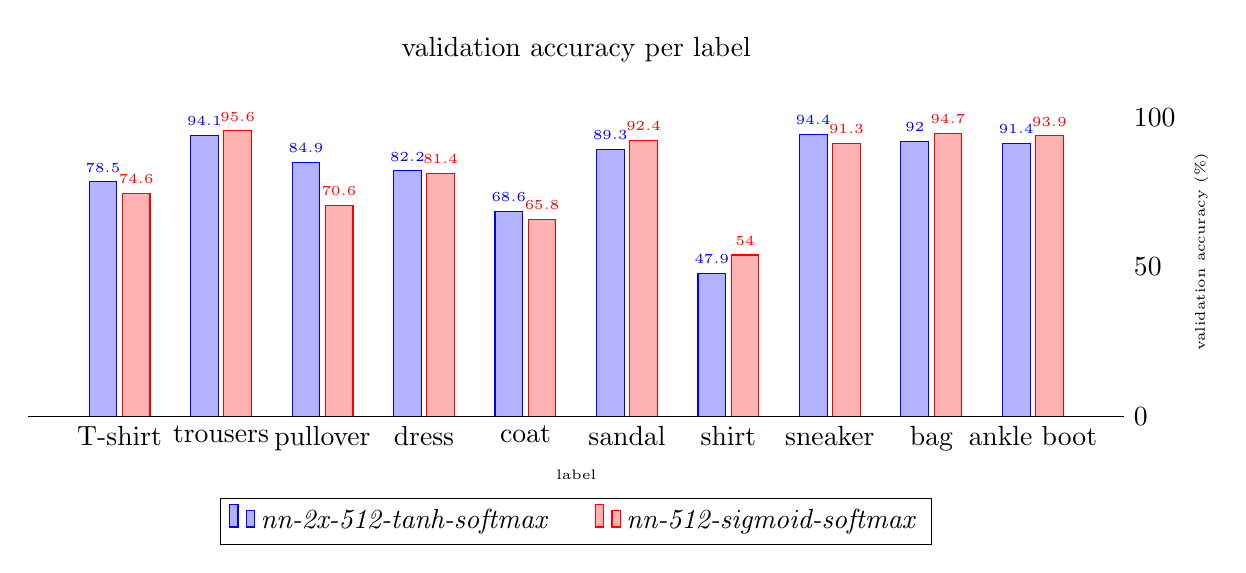
\begin{tikzpicture}
        \begin{axis}[
            symbolic x coords={T-shirt,trousers,pullover,dress,coat,sandal,shirt,sneaker,bag,ankle boot},
            width=15.5cm,
            height=5.75cm,
            ymax=100,
            ymin=0,
            xtick=data,
            ybar, axis on top,
            title={validation accuracy per label},
            height=5.75cm, width=15.5cm,
            tick align=inside,
            enlarge y limits={value=.1,upper},
            axis x line*=bottom,
            axis y line*=right,
            y axis line style={opacity=0},
            tickwidth=0pt,
            enlarge x limits=true,
            legend style={
                at={(0.5,-0.25)},
                anchor=north,
                legend columns=-1,
                /tikz/every even column/.append style={column sep=0.5cm}
           },
           ylabel={validation accuracy (\%)},
           xtick=data,
           xlabel={label},
           label style={font=\tiny},
           every node near coord/.append style={font=\tiny},
           nodes near coords={
            \pgfmathprintnumber[precision=2]{\pgfplotspointmeta}
           }
        ]
            \addplot coordinates {
                (T-shirt, 78.50)
                (trousers, 94.10)
                (pullover, 84.90)
                (dress, 82.20)
                (coat, 68.60)
                (sandal, 89.30)
                (shirt, 47.90)
                (sneaker, 94.40)
                (bag, 92.00)
                (ankle boot, 91.40)
            };
            \addplot coordinates {
                (T-shirt, 74.60)
                (trousers, 95.60)
                (pullover, 70.60)
                (dress, 81.40)
                (coat, 65.80)
                (sandal, 92.40)
                (shirt, 54.00)
                (sneaker, 91.30)
                (bag, 94.70)
                (ankle boot, 93.90)
            };
            \legend{\textit{nn-2x-512-tanh-softmax},\textit{nn-512-sigmoid-softmax}}
        \end{axis}

    \end{tikzpicture}
    \caption{Validation accuracy per label for the best network configurations}
    \label{figure:experiments:classification:accuracy-per-class-best}
\end{figure}
\begin{figure}[H]
    \begin{minipage}{.5\textwidth}
        \centering
        \includegraphics[scale=0.5]{experiments/classification/tanh.png}
        \captionof{figure}{Accuracy pattern of \textit{nn-2x-512-tanh-softmax} }
        \label{fig:experiments:classification:best-tanh}
    \end{minipage}%
    \hspace{0.25cm}
    \begin{minipage}{.5\textwidth}
        \centering
        \includegraphics[scale=0.5]{experiments/classification/sigmoid.png}
        \captionof{figure}{Accuracy pattern of \textit{nn-512-sigmoid-softmax}}
        \label{fig:experiments:classification:best-sigmoid}
    \end{minipage}
\end{figure}
